\documentclass{article}

\usepackage[T1]{fontenc}

\usepackage{polski}
\usepackage[utf8]{inputenc}
\usepackage[polish]{babel}
\let\lll\undefined
\usepackage{amssymb}
\usepackage{amsmath}
\usepackage{algorithm}
\usepackage{algpseudocode}
\usepackage{graphicx}
\usepackage{floatpag}
\usepackage{subcaption}



\title{Pracownia z analizy numerycznej \\ Sprawozdanie do zadania P2.01}
\author{Mikołaj Słupiński}
\date{Wrocław, dnia 1 grudnia 2016 r.}

\begin{document}
  \maketitle
  \section{Wstęp}
    \paragraph{}Jedną z najpopularniejszych metod rozwiązywania równań jest metoda
    Newtona. Jest ona prosta w implementacji i stosunkowo efektywna. Co ciekawe na
    jej podstawie można budować wiele innych metod iteracyjnych. Dwie z nich,
    metoda Halleya oraz jej wariant - metoda quasi-Halleya są szczególnie ciekawe
    ze względu na wyższy od metody Newtona wskaźnik zbieżności. W kolejnych
    sekcjach postaram się dokładnie przeanalizować działanie obu metod.

  \section{Matematyczne podstawy metody Halleya}

    \paragraph{} Aby zgłębić temat metody Halleya, która jest pewnym wariantem
    metody Newtona, przeanalizujmy najpierw zasadę działania jej pierwowzoru.
    Kolejne przybliżenia pierwiastka równania nieliniowego w metodzie Newtona
    otrzymujemy, posługując się wzorem:

    \begin{equation}\label{eq:newton}
      x_{k+1} = x_{k} - \frac{f(x_{k})}{f'(x_{k})} \,.
    \end{equation}

    Niech
    \begin{equation*}
      g(x) = \frac{f(x)}{\sqrt[]{|f'(x)|}}\,.
    \end{equation*}
    wtedy

    \begin{equation*}
      g'(x) = \frac{2[f'(x)]^2 - f(x)f''(x)}{2f'(x) \cdot \sqrt[]{|f'(x)|}}\,,
    \end{equation*}

    \begin{equation*}
      \frac{g(x)}{g'(x)}
      = \frac{f(x)}{\sqrt[]{f'(x)}} \cdot \frac{2f'(x) \cdot \sqrt[]{|f'(x)|}}{2(f'(x))^2 - f(x)f''(x)}
      = \frac{2f(x)f'(x)}{2(f'(x))^2 - f(x)f''(x)}
      = \frac{f(x)}{f'(x) - \frac{f(x)f''(x)}{2f'(x)}}\,.
    \end{equation*}

    Korzystając ze wzoru \eqref{eq:newton}, otrzymujemy:
    \begin{equation}\label{eq:halley}
      x_{k+1} = x_{k} - \frac{f(x_k)}{f'(x_k) - \frac{f(x_k)f''(x_k)}{2f'(x_k)}}\,.
    \end{equation}

    Równanie \eqref{eq:halley} pokazuje nam jak znajdować kolejne przybliżenia
    rozwiązań równań nieliniowych za pomocą metody Halleya.

    W metodzie siecznych przybliżamy korzystamy z faktu, że
    \begin{equation*}
      f'(x_k) \approx \frac{f(x_k) - f(x_{k-1})}{x_k - x_{k-1}}\,.
    \end{equation*}
    Zauważmy, że druga pochodna funkcji $f(x)$ jest tym samym, co pochodna funkcji
    $f'(x)$, zatem

    \begin{equation}\label{eq:halleyapprox}
      \frac{f(x_k)}{f'(x_k) - \frac{f(x_k)f''(x_k)}{2f'(x_k)}} \approx \frac{f(x_k)}{f'(x_k) - \frac{f'(x_k) - f'(x_{k-1})}{2(x_k - x_{k-1})f'(x_k)}f(x_k)} \,.
    \end{equation}

    Korzystając z wzorów \eqref{eq:halley} i \eqref{eq:halleyapprox} otrzymujemy
    metodę iteracyjną quasi-Halleya:

    \begin{equation*}
      x_{k+1} = x_{k} - \frac{f(x_k)}{f'(x_k) - \frac{f'(x_k) - f'(x_{k-1})}{2(x_k - x_{k-1})f'(x_k)}f(x_k)}\,.
    \end{equation*}

  \section{Przykłady obliczania pierwiastków równań metodami Halleya oraz quasi-Halleya}
  \label{sec:examples}

    \paragraph{} Spróbujmy teraz zastosować metody Halleya oraz quasi-Halleya do
    rozwiązania kilku równań nieliniowych. We wszystkich poniższych przykładach
    obliczenia wykonano programem \texttt{program.jl} z dokładnością $\varepsilon = 10^{-10}$.

    Zacznijmy od prostego równania nieliniowego
    \begin{equation*}
      e^{x} - 1 = 0 \,.
    \end{equation*}

    \begin{figure}
      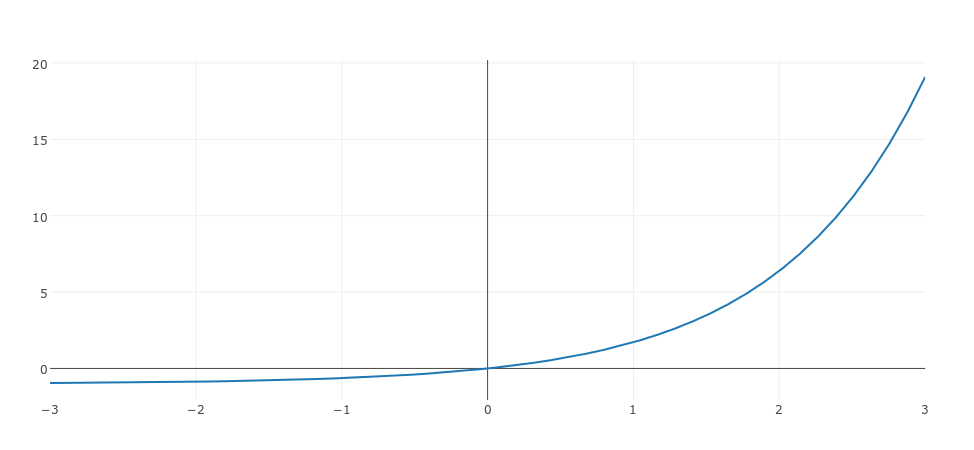
\includegraphics[width=\linewidth]{fplot.png}
      \caption{Wykres funkcji $f(x)$}
      \label{fig:fplot}
    \end{figure}

    Niech $f(x)$ będzie funkcją zadaną przez to równanie. Wtedy
    \begin{equation*}
      \begin{cases}
        f(x)   &= e^{x} - 1 \\
        f'(x)  &= e^{x}     \\
        f''(x) &= e^{x}     \\
      \end{cases}\,.
    \end{equation*}
    Jak łatwo zauważyć, równanie ma tylko jedno rozwiązanie $x = 0$.

    \begin{table}[!htb]
      \caption{Wartości kolejnych przybliżeń funkcji $f(x)$}
      \label{tab:f}

      \begin{subtable}{\linewidth}
        \centering
        \caption{Metoda Halleya}
        \label{tab:fa}
        \begin{tabular}{|l|l|l|l|}
          \hline
          $n$ & $x_n$                       & $f(x_n)$                    & $e_n$                       \\ \hline
          0   & 6.0                         & 402.4287934927              & 6.0                         \\
          1   & 4.0098904926                & 54.1408319052               & 4.0098904926                \\
          2   & 2.0811398821                & 7.0135982677                & 2.0811398821                \\
          3   & 0.5249138203                & 0.6903131714                & 0.5249138203                \\
          4   & 0.0117295719                & 0.0117986331                & 0.0117295719                \\
          5   & 1.3448048416 \cdot 10^{-7 } & 1.3448049319 \cdot 10^{-7 } & 1.3448048416 \cdot 10^{-7 } \\
          6   & 1.3265250638 \cdot 10^{-17} & 0.0                         & 1.3265250638 \cdot 10^{-17} \\
          \hline
        \end{tabular}
      \end{subtable}
      \begin{subtable}{\linewidth}
        \centering
        \caption{Metoda quasi-Halleya}
        \label{tab:fb}
        \begin{tabular}{|l|l|l|l|}
          \hline
          $n$ & $x_n$                       & $f(x_n)$                    & $e_n$                       \\ \hline
          0   & 0.0                         & 0.0                         & 0.0                         \\
          1   & 4.0                         & 53.5981500331               & 4.0                         \\
          2   & 2.8838623197                & 16.8832106418               & 2.8838623197                \\
          3   & -4.2833993225               & -0.9862043137               & -4.2833993225               \\
          4   & -4.2723343839               & -0.9860508176               & -4.2723343840               \\
          5   & -2.3168813814               & -0.9014194582               & -2.3168813814               \\
          6   & 0.7237809719                & 1.0622156682                & 0.7237809719                \\
          7   & 0.1635101788                & 0.1776373421                & 0.1635101788                \\
          8   & -0.0043002699               & -0.0042910370               & -0.0043002699               \\
          9   & -8.2754800592 \cdot 10^{-7} & -8.2754766350 \cdot 10^{-7} & -8.2754800593 \cdot 10^{-7} \\
          10  & 7.3222207818 \cdot 10^{-16} & 6.6613381478 \cdot 10^{-16} & 7.3222207818 \cdot 10^{-16} \\
          \hline
        \end{tabular}
      \end{subtable}
    \end{table}

    W tabeli~nr~\ref{tab:f} zestawiono kolejne przybliżenia miejsca zerowego funkcji
    $f(x)$, przedstawionej na wykresie~nr~\ref{fig:fplot}.

    \begin{figure}
      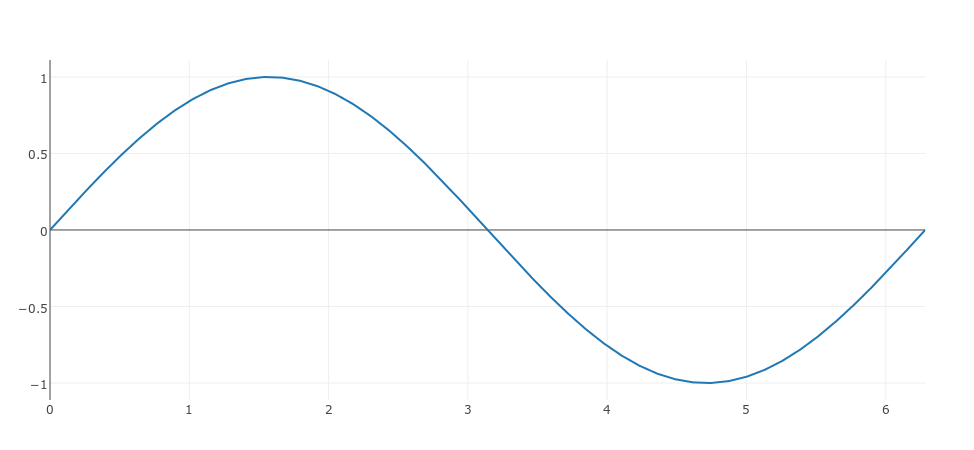
\includegraphics[width=\linewidth]{gplot.png}
      \caption{Wykres funkcji $g(x)$}
      \label{fig:gplot}
    \end{figure}

    Przyjrzymy się teraz mniej trywialnemu przypadkowi. Niech

    \begin{equation*}
      \begin{cases}
        g(x)   &= \sin x  \\
        g'(x)  &= \cos x  \\
        g''(x) &= -\sin x \\
      \end{cases}\,,
    \end{equation*}
    wtedy funkcja $g(x) = 0$ dla $x = k\pi$, gdzie $k \in \mathbb{Z}$. W tabeli~nr~\ref{tab:g}
    pokazano wyniki kolejnych przybliżeń argumentu funkcji. Jak widać, metoda
    Halleya z powodzeniem radzi sobie z wyznaczaniem pierwiastków równań o
    nieskończonej liczbie rozwiązań.

    \begin{table}[!htb]
      \caption{Wartości kolejnych przybliżeń funkcji $g(x)$}
      \label{tab:g}

      \begin{subtable}{\linewidth}
        \centering
        \caption{Metoda Halleya}
        \label{tab:ga}
        \begin{tabular}{|l|l|l|l|}
          \hline
          $n$ & $x_n$        & $g(x_n)$                     & $e_n$                        \\ \hline
          0   & 5.0          & -0.9589242747                & -1.2831853072                \\
          1   & 5.5035068196 & -0.7030508153                & -0.7796784876                \\
          2   & 6.1675976661 & -0.1153304281                & -0.1155876410                \\
          3   & 6.2829255094 & -0.0002597978                & -0.0002597978                \\
          4   & 6.2831853072 & -2.9223519302 \cdot 10^{-12} & -2.9221070008 \cdot 10^{-12} \\
          \hline
        \end{tabular}
      \end{subtable}
      \begin{subtable}{\linewidth}
        \centering
        \caption{Metoda quasi-Halleya}
        \label{tab:gb}
        \begin{tabular}{|l|l|l|l|}
          \hline
          $n$ &        $x_n$ & $g(x_n)$                     & $e_n$                        \\ \hline
          0   & 0.0          & 0.0                          & -9.4247779608                \\
          1   & 8.0          & 0.9893582466                 & -1.4247779608                \\
          2   & 9.5646557320 & -0.1394220807                & 0.1398777712                 \\
          3   & 9.4182387156 & 0.0065391986                 & -0.0065392452                \\
          4   & 9.4247794775 & -1.5167109112 \cdot 10^{-6 } & 1.5167109115  \cdot 10^{-6 } \\
          5   & 9.4247779608 & 3.9201077185  \cdot 10^{-15} & -3.5527136788 \cdot 10^{-15} \\
          \hline
        \end{tabular}
      \end{subtable}
    \end{table}

    \begin{figure}
      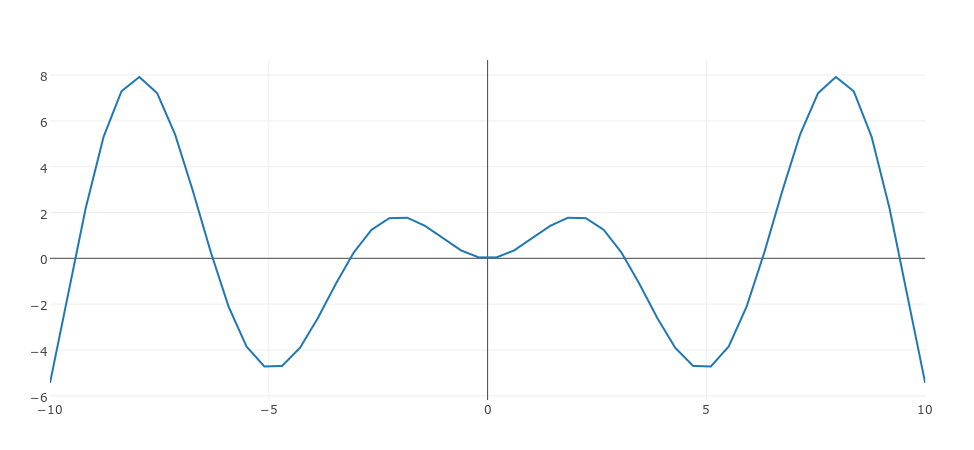
\includegraphics[width=\linewidth]{hplot.png}
      \caption{Wykres funkcji $h(x)$}
      \label{fig:hplot}
    \end{figure}

    Sprawdźmy teraz jak metoda Halleya radzi sobie z podwójnym
    miejscem zerowym. Niech

    \begin{equation*}
      \begin{cases}
        h(x)   &= x\sin x  \\
        h'(x)  &= \sin x + x\cos x  \\
        h''(x) &= 2\cos x - x\sin x \\
      \end{cases}\,,
    \end{equation*}
    wtedy funkcja ma podwójne zero w punkcie $x = 0$.

    Jak widać w tabeli~nr~\ref{tab:ha}, metoda zbiega do pierwiastka
    zdecydowanie wolniej niż w przypadku poprzednich funkcji.

    W tabeli~nr~\ref{tab:hb} pokazano, że dla metody quasi-Halleya uzyskano
    zbieżność do innego pierwiastka, mianowicie $x = 3\pi$.

    \begin{table}[!htb]
      \caption{Wartości kolejnych przybliżeń funkcji $h(x)$}
      \label{tab:h}

      \begin{subtable}{\linewidth}
        \centering
        \caption{Metoda Halleya}
        \label{tab:ha}
        \begin{tabular}{|l|l|l|l|}
          \hline
          $n$ & $x_n$                      & $h(x_n)$                    & $e_n$                      \\ \hline
          0   & 1.77                       & 1.7349973168                & 1.77                       \\
          1   & 1.2832128215               & 1.2305139389                & 1.2832128215               \\
          2   & 0.5289255934               & 0.2668990513                & 0.5289255934               \\
          3   & 0.1770906973               & 0.0311974520                & 0.1770906973               \\
          4   & 0.0590332729               & 0.0034829035                & 0.0590332729               \\
          5   & 0.0196777700               & 0.0003871896                & 0.0196777700               \\
          6   & 0.0065592567               & 4.3023540287 \cdot 10^{-5 } & 0.0065592567               \\
          7   & 0.0021864189               & 4.7804238361 \cdot 10^{-6 } & 0.0021864189               \\
          8   & 0.0007288063               & 5.3115858018 \cdot 10^{-7 } & 0.0007288063               \\
          9   & 0.0002429354               & 5.9017624664 \cdot 10^{-8 } & 0.0002429354               \\
          10  & 8.0978478104 \cdot 10^{-5} & 6.5575139089 \cdot 10^{-9 } & 8.0978478104 \cdot 10^{-5} \\
          11  & 2.6992826035 \cdot 10^{-5} & 7.2861265726 \cdot 10^{-10} & 2.6992826035 \cdot 10^{-5} \\
          12  & 8.9976086783 \cdot 10^{-6} & 8.0956961926 \cdot 10^{-11} & 8.9976086783 \cdot 10^{-6} \\
          \hline
        \end{tabular}
      \end{subtable}
      \begin{subtable}{\linewidth}
        \centering
        \caption{Metoda quasi-Halleya}
        \label{tab:hb}
        \begin{tabular}{|l|l|l|l|}
          \hline
          $n$ & $x_n$          & $h(x_n)$                     & $e_n$          \\ \hline
          0   & -1.77          & 1.7349973168                 & -11.1947779608 \\
          1   & 1.77           & 1.7349973168                 & -7.6547779608  \\
          2   & -10.6362159070 & -9.9568026953                & -20.0609938677 \\
          3   & -8.3363896665  & 7.3850439865                 & -17.7611676273 \\
          4   & -10.2327502307 & -7.3971279446                & -19.6575281915 \\
          5   & -9.1101289928  & 2.8194272464                 & -18.5349069536 \\
          6   & -9.4510842677  & -0.2485944492                & -18.8758622285 \\
          7   & -9.4247249590  & 0.0004995271                 & -18.8495029198 \\
          8   & -9.4247779608  & -1.7486431241 \cdot 10^{-10} & -18.8495559216 \\
          9   & -9.4247779608  & 3.4626072487 \cdot 10^{-15}  & -18.8495559215 \\
          \hline
        \end{tabular}
      \end{subtable}
    \end{table}

    \begin{figure}
      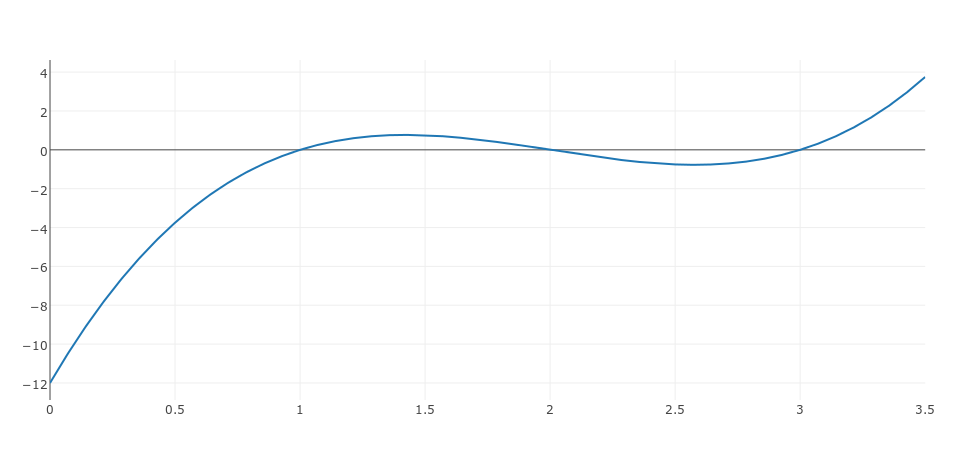
\includegraphics[width=\linewidth]{wplot.png}
      \caption{Wykres funkcji $w(x)$}
      \label{fig:wplot}
    \end{figure}

    Za ostatni przykład posłuży nam wielomian zdefiniowany następująco:

    \begin{equation*}
      \begin{cases}
        w(x)   &= 2x^3 - 12x^2 + 22x -12 \\
        w'(x)  &= 6x^2 - 24x + 22        \\
        w''(x) &= 12x - 24               \\
      \end{cases}\,.
    \end{equation*}

    W tabeli~nr~\ref{tab:w} pokazano wyniki kolejnych przybliżeń.

    \begin{table}[!htb]
      \caption{Wartości kolejnych przybliżeń funkcji $w(x)$}
      \label{tab:w}

      \begin{subtable}{\linewidth}
        \centering
        \caption{Metoda Halleya}
        \label{tab:wa}
        \begin{tabular}{|l|l|l|l|}
          \hline
          $n$ & $x_n$         & $w(x_n)$                    & $e_n$                        \\ \hline
          0   & -10.0         & -3432.0                     & -11.0                        \\
          1   & -4.0347945316 & -427.4896977498             & -5.0347945316                \\
          2   & -1.0870091171 & -52.6620620671              & -2.0870091171                \\
          3   & 0.3173064284  & -6.1635640490               & -0.6826935716                \\
          4   & 0.8860543540  & -0.5366430974               & -0.1139456460                \\
          5   & 0.9981690031  & -0.0073441153               & -0.0018309969                \\
          6   & 0.9999999893  & -4.2717621440 \cdot 10^{-8} & -1.0679405360 \cdot 10^{-8 } \\
          7   & 0.9999999999  & 0.0                         & -2.2204460493 \cdot 10^{-16} \\
          \hline
        \end{tabular}
      \end{subtable}
      \begin{subtable}{\linewidth}
        \centering
        \caption{Metoda quasi-Halleya}
        \label{tab:wb}
        \begin{tabular}{|l|l|l|l|}
          \hline
          $n$ & $x_n$         & $w(x_n)$                    & $e_n$                        \\ \hline
          0   & -10.0         & -3432.0                     & -11.0                        \\
          1   & -8.0          & -1980.0                     & -9.0                         \\
          2   & -2.7822178350 & -209.1704533163             & -3.7822178350                \\
          3   & 0.3576754160  & -5.5748052356               & -0.6423245840                \\
          4   & 1.2013402584  & 0.5784574581                & 0.2013402584                 \\
          5   & 1.0618024663  & 0.2247647107                & 0.0618024663                 \\
          6   & 1.0000234762  & 9.3901343634 \cdot 10^{-5 } & 2.3476162597  \cdot 10^{-5 } \\
          7   & 0.9999999999  & -1.020623586 \cdot 10^{-10} & -2.5515700663 \cdot 10^{-11} \\
          8   & 0.9999999999  & 0.0                         & -1.1102230246 \cdot 10^{-16} \\

          \hline
        \end{tabular}
      \end{subtable}
    \end{table}

  \section{Zbieżność metod Halleya oraz quasi-Halleya}

    \paragraph{}Metoda Halleya jest zbieżna sześciennie, natomiast wykładnik metody
    quasi-Halleya jest~$\ge 2.41$\cite{israel}. Możemy eksperymentalnie sprawdzić zbieżność powyższych
    metod.

    Do obliczenia wartości wykładnika zbieżności posłużymy się wzorem
    \begin{equation*}
      p \approx \frac{\log|\frac{x_{k+1} - x_k}{x_k - x_{k-1}}|}{\log|\frac{x_k - x_{k-1}}{x_{k-1} - x_{k-2}}|} \,,
    \end{equation*}
    gdzie $p$ jest wykładnikiem zbieżności naszego ciągu.

    W tabeli~nr~\ref{tab:convergence} zamieszczono wartości kolejnych przybliżeń $p_n$
    kolejnych przybliżeń wartości funkcji omówionych w sekcji~nr~\ref{sec:examples}.

    Jak można zaobserwować metoda Halleya w przypadku funkcji $f(x)$, $g(x)$ oraz $w(x)$
    osiąga zbieżność sześcienną, jednakże w przypadku funkcji $h(x)$ zbiega liniowo.
    Jest to spowodowane podwójnym zerem funkcji $h(x)$. Pierwsza pochodna tej funkcji
    jest zbieżna do zera w okolicy $x = 0$.

    Można zaobserwować duże wahania wartości wykładnika zbieżności metody quasi-Halleya,
    jednakże jego końcowe wartości w przypadku funkcji $f(x)$, $g(x)$ oraz $h(x)$
    znajdują się w okolicach 2.41, czyli są zgodne z oczekiwanymi.

    \begin{table}[htb]
      \centering
      \caption{Wartości wykładników zbieżności dla poszczególnych funkcji}
      \label{tab:convergence}
      \begin{tabular}{|r||r|r|r|r||r|r|r|r|}
        \hline
        \multicolumn{5}{|c||}{Halley}              & \multicolumn{4}{|c|}{quasi-Halley}   \\ \hline \hline
        $n$ & $f(x)$ & $g(x)$  & $h(x)$  & $w(x)$ & $f(x)$  & $g(x)$ & $h(x)$  & $w(x)$  \\ \hline
        0   & 6.8527 & -6.3241 & -1.7413 & 1.0519 & -1.4569 & 1.4518 & -1.3439 & -0.5296 \\
        1   & 5.1693 &  3.4819 &  1.4319 & 1.2190 & -3.4810 & 1.3121 &  0.1145 &  2.5876 \\
        2   & 3.4060 &         &  1.0059 & 1.7966 & -0.7994 & 2.6925 &  2.7179 &  1.3692 \\
        3   & 3.0107 &         &  1.0000 & 2.5338 &  0.0853 &        &  2.2730 &  0.4528 \\
        4   &        &         &  1.0000 & 2.9290 & -3.8315 &        &  2.1482 &  9.6658 \\
        5   &        &         &  1.0000 &        &  0.7128 &        &  2.4256 &  1.7437 \\
        6   &        &         &  1.0000 &        &  3.0395 &        &  2.3940 &         \\
        7   &        &         &  1.0000 &        &  2.3348 &        &         &         \\
        8   &        &         &  1.0000 &        &         &        &         &         \\
        9   &        &         &  1.0000 &        &         &        &         &         \\
        \hline
      \end{tabular}
    \end{table}


  \section{Wnioski}

    \paragraph{} Metoda Halleya charakteryzuje się sześcienną zbieżnością, co czyni
    ją niezwykle wydajną metodą iteracyjną rozwiązywania równań. Jednakże nie jest
    ona pozbawiona wad. Aby ją zastosować musimy znać pierwszą oraz drugą pochodną
    funkcji. Pomijając trudności z obliczeniem pochodnej, funkcja może nie posiadać
    drugiej pochodnej lub w ogóle nie być różniczkowalna. Nawet ciągłość funkcji
    może nie być warunkiem wystarczającym, do jej rozwiązalności, za przykład może
    nam posłużyć piła Weierstrassa, która jest ciągła, ale nie jest różniczkowalna
    w żadnym punkcie.

    Natomiast metodaa quasi-Halleya okazuje się sensowną alternatywą dla standardowej
    metody Newtona. Jej zbieżność jest znacząco lepsza od kwadratowej zbiezności
    metody Newtona i podobnie jak ona wymaga znania jedynie pierwszej pochodnej.
    \begin{thebibliography}{9}
      \bibitem{kincaid}
        David Kincaid, Ward Cheney,
        \textit{Analiza Numeryczna},
        Wydawnictwa Naukowo-Techniczne, Warszawa, 2006.

      \bibitem{bjorck}
        Ake Bjorck, Germund Dahlquist,
        \textit{Metody numeryczne},
        Państwowe Wydawnictwo Naukowe, 1987.

      \bibitem{israel}
        A. Ben-Israel:  LU factorization,
        \textit{Newton’s Method with Modified Functions},
        Contemporary Mathematics 204 (1997), 39–50.
    \end{thebibliography}


\end{document}
